\documentclass[a4paper,11pt]{book}
\renewcommand{\familydefault}{\sfdefault}

\usepackage{standalone}
\usepackage[english]{babel}
\usepackage[top=3cm]{geometry}
\usepackage{float}
\usepackage{tabularx}
\usepackage{multirow}
\usepackage{booktabs}
\usepackage{pgfplots}
\usepackage{amsmath}
\usepackage{amssymb}
\usepackage{amsfonts}
\usepackage{siunitx}
\usepackage{tikz}
\usepackage{graphics} % for pdf, bitmapped graphics files
\usepackage{graphicx}
\usepackage{exsheets}
\usepackage{algorithm}
\usepackage{algorithmicx}
\usepackage[noend]{algpseudocode}
\usepackage{hyperref}
\usepackage{enumitem}
\usepackage{filecontents}
\usepackage{multirow}
%\usepackage{showframe}% to show frames
%\ifCLASSOPTIONcompsoc
\usepackage[caption=false, font=normalsize, labelfont=sf, textfont=sf]{subfig}
%\else
%\usepackage[caption=false, font=footnotesize]{subfig}
%\fi    

\usetikzlibrary{patterns,arrows,arrows.meta,calc,intersections,shapes,positioning,decorations.pathreplacing,decorations.markings,decorations.pathmorphing}
\usepackage{multicol}

\sisetup{output-decimal-marker={,},exponent-product=\cdot}

\DeclareSIUnit\atm{atm}
\DeclareSIUnit\dioptre{D}



\def\BState{\State\hskip-\ALG@thistlm}


\definecolor{TitleColor}{rgb}{0.65,0.04,0.07}
\definecolor{NumberColor}{rgb}{0.02,0.04,0.48}

\DeclareInstance{exsheets-heading}{fancy}{default}{
toc-reversed = true ,
indent-first = true ,
vscale = 2 ,
pre-code = \IfInsideQuestionT{\rule{\linewidth}{1pt}} ,
post-code =\IfInsideQuestionT{\rule{\linewidth}{1pt}} ,
subtitle-format = \large\scshape\color{rgb:red,0.65;green,0.04;blue,0.07} ,
number-format = \large\bfseries\color{rgb:red,0.02;green,0.04;blue,0.48} ,
points-format = \itshape ,
join = { number[r,B]title[l,B](.333em,0pt);
title[r,B]subtitle[l,B](1em,0pt)
} ,
attach =
{
main[hc,vc]number[hc,vc](0pt,0pt) ;
main[l,vc]subtitle[hc,vc](\marginparsep,0pt)
}
}



\DeclareInstance{exsheets-heading}{block-subtitle}{default}{
vscale = 2 ,
pre-code = \rule{\linewidth}{1pt} ,
post-code = \rule{\linewidth}{1pt} ,%title-format = \large\scshape\color{TitleColor} ,
number-format = \large\bfseries\color{rgb:red,0.02;green,0.04;blue,0.48} ,
subtitle-format = \large\scshape\color{black} ,
join = {
title[r,B]number[l,B](.333em,0pt) ;
title[r,B]subtitle[l,B](1em,0pt)
} ,
attach = {
main[l,vc]title[l,vc](0pt,0pt) ;
main[r,vc]points[l,vc](\marginparsep,0pt)
},
}

\DeclareQuestionClass{textbook}{textbooks}

\SetupExSheets{
  headings = fancy,
  question/print = true ,
  solution/print = false }
 % counter-format = se.qu ,
%  counter-within = section ,
  %question/pre-hook = \rule{\textwidth}{1pt},


\hypersetup{
	colorlinks = true, 
	breaklinks = true, 
	bookmarks = true,
	bookmarksnumbered = true,
	urlcolor = blue, 
	linkcolor = blue, 
	citecolor=blue,
	linktoc=page, 
	pdftitle={}, 
	pdfauthor={\textcopyright Author}, 
	pdfsubject={}, 
	pdfkeywords={}, 
	pdfcreator={pdfLaTeX}, % PDF Creator
	pdfproducer={IEEE} }





\tikzset{point/.style={circle,fill,black!80,inner sep=0pt,minimum size=#1,opacity=0.9}}
\tikzset{point/.default=3pt}\tikzset{vector/.style={line width=1pt,postaction={decorate,decoration={markings,mark=at position 1 with {\arrow{latex}}}}}}
\tikzset{block/.style={rectangle,fill=black!30,draw,minimum size=#1,opacity=0.9,align=center}}
\tikzset{block/.default=15pt}\tikzset{ball/.style={circle,fill=black!30,draw,minimum size=#1,opacity=0.9}}
\tikzset{ball/.default=5pt}\tikzset{pulley/.style={draw=black,line width=0.2pt,circle,minimum size=#1,inner sep=0pt,fill=black!10}}
\tikzset{pulley/.default=20pt}\tikzset{rod/.style={line width=2pt}}
\tikzset{rope/.style={line width=1pt}}
\tikzset{spring/.style={decorate,decoration={coil,amplitude=5pt,segment length=#1,aspect=0.3}}}
\tikzset{spring/.default=5pt}\tikzset{wall/.style={black!10,pattern=north east lines,opacity=0.3}}
\tikzset{ray/.style={line width=0.8pt,postaction={decorate,decoration={markings,mark=at position 0.5 with {\arrow{>}}}}}}
\tikzset{arrow/.style={-latex}}
\tikzset{object/.style={line width=1pt,orange,-latex}}
\tikzset{image/.style={line width=1pt,blue,-latex}}
\tikzset{doublearrow/.style={<->,>=latex,thick}}
\tikzset{brace/.style={decorate,decoration={brace,amplitude=#1}}}
\tikzset{brace/.default=5pt}




\graphicspath{{images/}} 




\makeatletter
\@addtoreset{question}{section}
\makeatother


\begin{document}
\author{Dr. Muhammed Rushdi \and Asem Alaa}

\title{Measurements and Instrumentation [SBE206A] (Fall 2018)\\ Tutorial 6 (Revision Problems)}

\maketitle


\section*{Problems on first-order systems}


\begin{question}

Output variable $y$ responds like a first-order dynamic system when exposed to a sudden change of input variable x. The half-life of the system is $2.00$ s. When $x$ is suddenly
increased, $y$ grows from an initial value of $100$ to a final value of $132$.
Calculate the time (in seconds) required for $y$ to reach a value of $124$.
\examspace*{10em}

\end{question}
\begin{solution}


\end{solution}

\chapter*{Typical 2\textsuperscript{nd}-order systems}


\section*{Second-order spring-mass-damper system}


\begin{figure*}[h!]\label{fig:damper}
\centering
  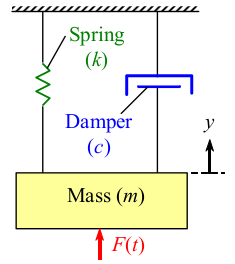
\includegraphics[width=0.3\linewidth]{damper}
  \caption{Second-order spring-mass-damper system.} 
\end{figure*}

\subsection*{Derivation of the 2\textsuperscript{nd}-order equation}

By applying Newton's second law, on the free body diagram in \ref{fig:freebody}:

\begin{figure*}[h!]\label{fig:freebody}
\centering
  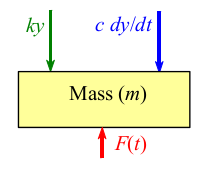
\includegraphics[width=0.3\linewidth]{newton}
  \caption{Free body diagram.} 
\end{figure*}

\begin{align}
\sum F &= m a \\ 
F_{\rm spring} + F_{\rm damper} + F_{\rm input}(t) &= m \frac{d^2y}{dt^2} \\ 
-ky -c \frac{dy}{dt} + F_{\rm input}(t) &= m \frac{d^2y}{dt^2} \label{eqn:mass-spring}
\end{align}

Applying Laplace transform on Eqn ~\ref{eqn:mass-spring}:

\begin{align*}
-kY(s) - c\left[sY(s)-y(0)\right] + F(s) &= m\left[s^2Y(s)-y'(0)-sy(0)\right] \\
F(s) + y(0) + my'(0)+msy(0) &= \left[ms^2+cs+k\right]Y(s) \\
Y(s) &= \frac{F(s) + y(0) + my'(0)+msy(0)}{ms^2+cs+k} \\
&= \frac{F(s)/m + y(0)/m + y'(0)+sy(0)}{s^2+\frac{c}{m}s+ \frac{k}{m}}
\end{align*}

By equating the denumerator to the characteristic polynomial of the 2\textsuperscript{nd}-order system $N(s)=(s^2 + 2 \eta \omega_n s + {\omega_n}^2)$, we realize that:
\begin{itemize}
\item $\omega_n=\sqrt{\frac{k}{m}}$
\item $\eta = \frac{c}{\sqrt{km}}$
\end{itemize} 



\section*{Problems on 2\textsuperscript{nd}-order systems}


\begin{question}

A spring-mass-damper system is set up with the following
properties: mass $m = 22.8$g, spring constant $k = 51.6$ N/cm, and damping coefficient $c = 3.49 $ N$\cdot$s/m. The forcing function is a step function (sudden jump).
\begin{enumerate}
\item Calculate the damping ratio of this system. Will it oscillate?
\item If the system will oscillate, calculate the oscillation frequency in hertz. [Note: Calculate the physical frequency, not the radian frequency.] Compare the actual oscillating frequency to the undamped natural frequency of the system.
\end{enumerate}
\examspace*{10em}

\end{question}
\begin{solution}


\end{solution}

\begin{question}

The following second-order ODE:
\begin{equation*}
5\frac{d^2y}{dt^2} + \frac{dy}{dt} + 1000y= x(t)
\end{equation*}
The forcing function is a step function (sudden jump):
\begin{itemize}
\item $x(t) = 0$ for $t<0$
\item $x(t) = 25$ for $t>0$
\end{itemize}


\begin{enumerate}
\item Calculate the natural frequency and damping ratio of this system.
\item Calculate the equilibrium response (as $t \to \infty$ , what is $y$?)
\end{enumerate}

\examspace*{10em}

\end{question}
\begin{solution}


\end{solution}



\begin{question}

\begin{figure*}[h!]\label{fig:freebody}
\centering
  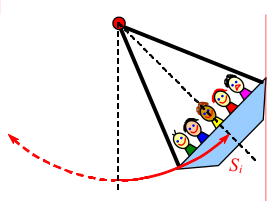
\includegraphics[width=0.3\linewidth]{penduleum}
  \caption{A pendulum-type system.} 
\end{figure*}

A pendulum-type amusement park ride
behaves as a 2\textsuperscript{nd}-order dynamic system with damping ratio $\eta = 0.1$ and $f_n = 0.125$ Hz. For an initial displacement $S_i = 10.0$ m, calculate the damped natural frequency, the undamped natural frequency, and how long it takes for the oscillations to damp out to within 5\% of $S_i$ (the 95\% response time).

\examspace*{10em}

\end{question}
\begin{solution}


\end{solution}



\end{document}
